\documentclass{beamer}

\usetheme[subsection page=progressbar]{metropolis}
\usepackage{appendixnumberbeamer}

\usepackage{amsmath}
\usepackage{amssymb}
\usepackage{amsthm}
\usepackage{mathtools}
\usepackage{bussproofs}
\usepackage{stmaryrd}
\usepackage{gb4e}
\noautomath
\usepackage{url}
\usepackage{subcaption}
\usepackage{array}
\usepackage[toc,page]{appendix}
\usepackage[export]{adjustbox}[2011/08/13]
\usepackage{rotating}
\usepackage{tikz}
\usepackage{tikz-qtree}
\usepackage{etoolbox}
\usepackage{chngpage}
\usepackage{fancybox}
\usepackage{enumerate}
\usepackage{drs}
\input{qobitree}
\usepackage{forest}
\usepackage{color}
\usepackage{graphicx}


\newcommand{\hsbind}{\mathbin{\gg\!=}}
\newcommand{\apl}{\mathbin{\ll\!\!\cdot}}
\newcommand{\apr}{\mathbin{\cdot\!\!\gg}}
\newcommand{\aplr}{\mathbin{\ll\!\!\cdot\!\!\gg}}
\newcommand{\cons}{\mathbin{::}}
\newcommand{\cat}{\mathbin{+\mkern-10mu+}}

\newcommand{\abs}[1]{\textsc{#1}}
\newcommand{\obj}[1]{\textbf{#1}}
\newcommand{\sem}[1]{\llbracket #1 \rrbracket}
\newcommand{\lex}[2]{\sem{\abs{#1}} &:= #2}

\newcommand{\dand}{\mathbin{\overline{\land}}}
\newcommand{\dnot}{\mathop{\overline{\lnot}}}
\newcommand{\dor}{\mathop{\overline{\lor}}}
\newcommand{\dimpl}{\mathbin{\overline{\to}}}
\newcommand{\dexists}{\mathop{\overline{\exists}}}
\newcommand{\dforall}{\mathop{\overline{\forall}}}

\newcommand{\limp}{\mathbin{{-}\mkern-3.5mu{\circ}}}

\newcommand{\llbparenthesis}{\vcenter{\hbox{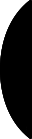
\includegraphics{symbols/llbparenthesis.png}}}}
\newcommand{\rrbparenthesis}{\vcenter{\hbox{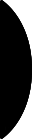
\includegraphics{symbols/rrbparenthesis.png}}}}
\newcommand{\lban}{\llparenthesis \,}
\newcommand{\rban}{\, \rrparenthesis}
\newcommand{\lbban}{\llbparenthesis \,}
\newcommand{\rbban}{\, \rrbparenthesis}
\newcommand{\banana}[1]{\lban #1 \rban}
\newcommand{\bbanana}[1]{\lbban #1 \rbban}
\newcommand{\cherry}{\rotatebox[origin=c]{270}{$\limp$}}

\newcommand{\lam}[2]{\lambda #1.\, #2}
\newcommand{\ap}[2]{#1\,#2}
\newcommand{\app}[3]{\ap{\ap{#1}{#2}}{#3}}
\newcommand{\appp}[4]{\ap{\ap{\ap{#1}{#2}}{#3}}{#4}}
\newcommand{\op}[1]{\mathtt{#1}}
\newcommand{\onto}[1]{#1 \mathalpha{:\,}}
\newcommand{\typedop}[3]{\op{#1} : #2 \rightarrowtail #3}
\newcommand{\typedopg}[3]{#1 : #2 \rightarrowtail #3}
\newcommand{\row}[2]{\{ #1 \mathrel{|} #2 \}}

\newcommand{\CC}{\mathcal{C}}
\newcommand{\FF}{\mathcal{F}}
\newcommand{\XX}{\mathcal{X}}
\newcommand{\EE}{\mathcal{E}}
\newcommand{\TT}{\mathcal{T}}
\newcommand{\PP}{\mathcal{P}}

\newcommand{\FV}{\operatorname{FV}}

\newcommand{\subst}[3]{#1[#2 \coloneqq #3]}

\newcommand{\syntclos}[1]{\mathbin{[#1]}}

\newcommand{\cibanana}{\banana{(\onto{\op{op}_i} M_i)_{i \in I},\ \onto{\eta} M_\eta}}
\newcommand{\cdbanana}{\banana{\onto{\op{op}_1} M_1,\ \dots,\ \onto{\op{op}_n} M_n,\ \onto{\eta} M_\eta}}

\newcommand{\cibbanana}{\bbanana{(\onto{\op{op}_i} M_i)_{i \in I},\ \onto{\eta} M_\eta}}

\newcommand{\TODO}[1]{\textbf{TODO}: #1}

\newcommand{\relR}{\mathbin{R}}

\newcommand{\swap}{\mathbin{\textbf{swap}}}

\newcommand{\tto}{\twoheadrightarrow}

\mathchardef\mhyphen="2D

\newcommand{\pair}[2]{\left<#1, #2\right>}
\newcommand{\inl}{\operatorname{inl}}
\newcommand{\inr}{\operatorname{inr}}

\newcommand{\true}{\textbf{T}}
\newcommand{\false}{\textbf{F}}
\newcommand{\ifte}[3]{\text{\textbf{if} $#1$ \textbf{then} $#2$ \textbf{else} $#3$}}


% Examples
\newcommand{\expr}[1]{\textsc{#1}}
\newcommand{\sume}{\expr{sum}}
\newcommand{\prode}{\expr{prod}}
\newcommand{\lite}{\expr{lit}}
\newcommand{\dive}{\expr{div}}
\newcommand{\trye}{\expr{try}}
\newcommand{\lete}{\expr{let}}
\newcommand{\vare}{\expr{var}}
\newcommand{\sumecn}[2]{\app{\sume}{#1}{#2}}
\newcommand{\prodecn}[2]{\app{\prode}{#1}{#2}}
\newcommand{\litecn}[1]{\ap{\lite}{#1}}
\newcommand{\divecn}[2]{\app{\dive}{#1}{#2}}
\newcommand{\tryecn}[2]{\app{\trye}{#1}{#2}}
\newcommand{\letecn}[3]{\appp{\lete}{\bar{#1}}{#2}{#3}}
\newcommand{\varecn}[1]{\ap{\vare}{#1}}

\newcommand{\paren}[1]{(#1)}

\newcommand{\sumec}[2]{\paren{\sumecn{#1}{#2}}}
\newcommand{\prodec}[2]{\paren{\prodecn{#1}{#2}}}
\newcommand{\litec}[1]{\paren{\litecn{#1}}}
\newcommand{\divec}[2]{\paren{\divecn{#1}{#2}}}
\newcommand{\tryec}[2]{\paren{\tryecn{#1}{#2}}}
\newcommand{\letec}[3]{\paren{\letecn{#1}{#2}{#3}}}
\newcommand{\varec}[1]{\paren{\varecn{\bar{#1}}}}


\newcommand{\NN}{\mathbb{N}}
\newcommand{\dbze}{\frac{\cdot}{0}}
\newcommand{\dbzelong}{\operatorname{DivisionByZero}}


\newcommand{\reseto}{\mathtt{reset0}}
\newcommand{\shifto}{\mathtt{shift0}}
\newcommand{\resetobanana}{\banana{\onto{\op{shift0}}{(\lam{c k}{\ap{c}{k}})}}}
\newcommand{\resetbanana}{\bbanana{\onto{\op{shift0}}{(\lam{c k}{\ap{c}{k}})}}}
\newcommand{\from}{\leftarrow}

\newcommand*{\twoheadleftrightarrow}{%
  \twoheadleftarrow
  \mathrel{\mkern-15mu}%
  \twoheadrightarrow
}

\newcommand{\ffrom}{\twoheadleftarrow}
\newcommand{\ttoffrom}{\twoheadleftrightarrow}


\newcommand{\reset}{\mathtt{reset}}
\newcommand{\shift}{\mathtt{shift}}

\newcommand{\semo}[1]{\sem{#1}_0}


\newcommand{\demph}[1]{\textbf{#1}}

\newcommand{\pipe}{\mathbin{|}}
\newcommand{\xto}[1]{\xrightarrow{#1}}

\renewcommand\theequation{\arabic{equation}}


\definecolor{transparent}{RGB}{208,213,213}


\title{Introducing a Calculus of Effects and Handlers for Natural Language Semantics}
\date{August 20, 2016}
\author{Jirka Maršík \and Maxime Amblard}
\institute{LORIA, UMR 7503, Université de Lorraine, CNRS, Inria, Campus Scientifique, \\
F-54506 Vand\oe uvre-lès-Nancy, France \\
\textbf{jiri.marsik89@gmail.com}}


\begin{document}

\maketitle


\section{Introduction}


\begin{frame}{Fighting with Compositionality}
  \begin{block}{Setting}
    Formal Semantics
  \end{block}
  
  \pause
  \begin{block}{Compositionality}
    The \alert<6>{meaning} of a complex expression is a \alert<4>{function}
    of its structure and the \alert<6>{meanings} of its constituents.
  \end{block}
  
  \pause
  \begin{block}{Case of quantification}
  \begin{itemize}
  \item use $\lambda\mu$ \cite{de2001type} or $\shift$/$\reset$
    \cite{shan2005linguistic} \alert<4>{functions}
    \uncover<7>{\begin{flushright}\alert{calculi with effects}\end{flushright}}
  \pause
  \pause
  \item use continuized \alert<6>{meanings} \cite{barker2002continuations},
    i.e.\ generalized quantifiers
    \uncover<7>{\begin{flushright}\alert{term encodings of effects}\end{flushright}}
  \end{itemize}
  \end{block}
\end{frame}


\begin{frame}{Connections to Existing Work}
  \begin{block}{Pioneers}
  \begin{itemize}
  \item \cite{shan2002monads,hobbs1977making}
  \end{itemize}
  \end{block}
  
  \begin{block}{Parallel developments}
  \begin{itemize}
  \item \cite{charlow2014semantics,kiselyov2015swing}
  \end{itemize}
  \end{block}

  \begin{block}{ESSLLI courses}
  \begin{itemize}
  \item \cite{barker2015monads,giorgolo2015natural}
  \end{itemize}
  \end{block}
  
  \begin{block}{Effects and Handlers}
  \begin{itemize}
  \item
    \cite{cartwright1994extensible,plotkin2013handling,bauer2012programming,kammar2013handlers,kiselyov2013extensible}
  \end{itemize}
  \end{block}
\end{frame}


\section{Definition of the \texorpdfstring{$\calc$}{} Calculus}

\begin{frame}{STLC with Computations}

  Simply typed lambda calculus (STLC) with computation types $\FF_E(\gamma)$

  \vfill
  
  \begin{block}{Constructors for $\FF_E(\gamma)$}
   \begin{prooftree}
    \AxiomC{$\Gamma \vdash M : \gamma$}
    \RightLabel{[$\eta$]}
    \UnaryInfC{$\Gamma \vdash \ap{\eta}{M} : \FF_E(\gamma)$}
  \end{prooftree}

  \begin{prooftree}
    \AxiomC{$\Gamma \vdash M_{\mathrm{p}} : \alpha$}
    \AxiomC{$\Gamma, x : \beta \vdash M_{\mathrm{c}} : \FF_E(\gamma)$}
    \def\extraVskip{0pt}
    \noLine
    \BinaryInfC{$\typedop{op}{\alpha}{\beta} \in E$}
    \def\extraVskip{2pt}
    \RightLabel{[op]}
    \UnaryInfC{$\Gamma \vdash \app{\op{op}}{M_{\mathrm{p}}}{(\lam{x}{M_{\mathrm{c}}})} : \FF_E(\gamma)$}
  \end{prooftree}
  \end{block}
\end{frame}


\begin{frame}{Example Computation}

  \begin{align*}
    \Gamma \vdash\ &\app{\op{speaker}}{\star}{(\lam{s}{ \\
                 \ &\app{\op{implicate}}{(\obj{m} = \obj{best-friend}(s))}{(\lam{\_}{ \\
                 \ &\etaE{(\obj{love}(\obj{m}, s))}})}})} : \FF_E(o)
  \end{align*}

  \begin{align*}
    E = \{\ &\typedop{speaker}{1}{\iota}, \\
          \ &\typedop{implicate}{o}{1}\ \}
  \end{align*}

  \vfill
  \pause

  $$
  \sem{\text{Mary, my best friend, loves me.}}
  $$
\end{frame}


\begin{frame}{Computations as Programs}

  \begin{align*}
    \Gamma \vdash\ &\app{\op{speaker}}{\star}{(\lam{s}{ \\
                 \ &\app{\op{implicate}}{(\obj{m} = \obj{best-friend}(s))}{(\lam{\_}{ \\
                 \ &\etaE{(\obj{love}(\obj{m}, s))}})}})} : \FF_E(o)
  \end{align*}

  \vfill
  \centerline{$\Downarrow$}
  \vfill

  \begin{align*}
    \textrm{do}\ &s \from \ap{\op{speaker}}{\star} \\
                 &\ap{\op{implicate}}{(\obj{m} = \obj{best-friend}(s))} \\
                 &\textrm{return}\ (\obj{love}(\obj{m}, s))
  \end{align*}
\end{frame}


\begin{frame}{Computations as Algebraic Expressions}

  \begin{align*}
    \Gamma \vdash\ &\app{\op{speaker}}{\star}{(\lam{s}{ \\
                 \ &\app{\op{implicate}}{(\obj{m} = \obj{best-friend}(s))}{(\lam{\_}{ \\
                 \ &\etaE{(\obj{love}(\obj{m}, s))}})}})} : \FF_E(o)
  \end{align*}

  \vfill
  \centerline{$\Downarrow$}
  \vfill
 
  \hspace*{-8mm}
  \begin{forest}
    [$\op{speaker}\ (\star)$,draw,ellipse
      [$\op{impl.}\ (\obj{m} {=} \obj{bff}(\obj{a}))$,draw,ellipse,edge label={node[midway,left,xshift=-3mm] {$\obj{a}$}}
        [$\obj{love}(\obj{m}{,} \obj{a})$,draw,edge label={node[midway,left] {$\star$}}]]
      [$\op{impl.}\ (\obj{m} {=} \obj{bff}(\obj{b}))$,draw,ellipse,edge label={node[midway,left] {$\obj{b}$}}
        [$\obj{love}(\obj{m}{,} \obj{b})$,draw,edge label={node[midway,left] {$\star$}}]]
      [{$\ \hspace{5mm}\cdots\hspace{1cm}\ $},edge label={node[midway,left,xshift=-3mm] {$\ldots$}}]]
  \end{forest}
\end{frame}


\begin{frame}{Closed Handlers}

  \begin{prooftree}
  \AxiomC{$E = \{\typedopg{\op{op}_i}{\alpha_i}{\beta_i}\}_{i \in I}$}
  \def\extraVskip{2pt}
  \noLine
  \UnaryInfC{$[\Gamma \vdash M_i : \alpha_i \to (\beta_i \to \alert<3>{\delta}) \to \alert<3>{\delta}]_{i \in I}$}
  \noLine
  \UnaryInfC{$\Gamma \vdash M_\eta : \gamma \to \alert<3>{\delta}$}
  \noLine
  \UnaryInfC{$\Gamma \vdash N : \FF_E(\gamma)$}
  \def\extraVskip{4pt}
  \RightLabel{$[\bbanana{}]$}
  \UnaryInfC{$\Gamma \vdash \ap{\cibbanana}{N} : \delta$}
  \end{prooftree}

  \begin{columns}
  \pause
  \column{0.6\textwidth}
  \begin{block}{Types of constructors}
  \begin{itemize}
  \item $\op{op}_i : \alpha_i \to (\beta_i \to \alert<3>{\FF_E(\gamma)}) \to \alert<3>{\FF_E(\gamma)}$
  \item $\eta : \gamma \to \alert<3>{\FF_E(\gamma)}$
  \end{itemize}
  \end{block}

  \pause
  \pause
  \column{0.4\textwidth}
  \begin{block}{Handlers are algebras}
  \begin{itemize}
  \item $(\delta, M_i)$ --- an algebra
    \begin{itemize}
    \item $\delta$ --- carrier
    \item $M_i$ --- operations
    \end{itemize}
  \item $M_\eta$ --- constants
  \end{itemize}
  \end{block}
  \end{columns}
\end{frame}


\begin{frame}{Open Handlers}

  \begin{prooftree}
  \AxiomC{$E = \{\typedopg{\op{op}_i}{\alpha_i}{\beta_i}\}_{i \in I} \uplus E_{\mathrm{f}}$}
  \noLine
  \def\extraVskip{2pt}
  \UnaryInfC{$E' = E'' \uplus E_{\mathrm{f}}$}
  \noLine
  \UnaryInfC{$[\Gamma \vdash M_i : \alpha_i \to (\beta_i \to
    \FF_{E'}(\delta)) \to \FF_{E'}(\delta)]_{i \in I}$}
  \noLine
  \UnaryInfC{$\Gamma \vdash M_\eta : \gamma \to \FF_{E'}(\delta)$}
  \noLine
  \UnaryInfC{$\Gamma \vdash N : \FF_{E}(\gamma)$}
  \def\extraVskip{4pt}
  \RightLabel{[$\banana{}$]}
  \UnaryInfC{$\Gamma \vdash \ap{\cibanana}{N} : \FF_{E'}(\delta)$}
  \end{prooftree}

  \pause
  \begin{columns}
  \column{0.5\textwidth}
  \begin{itemize}
  \item $E$ --- input effects
  \item $E_\petitf$ --- forwarded effects
  \end{itemize}
  \column{0.5\textwidth}
  \begin{itemize}
  \item $E'$ --- output effects
  \item $E''$ --- new effects
  \end{itemize}
  \end{columns}
\end{frame}


\setbeamercovered{transparent=30}

\begin{frame}{Reduction Rules for Handlers}

  \begin{tabular*}{\textwidth}{l @{\extracolsep{\fill}} r}
  $\ap{\uncover<1,3>{\cibanana}}{(\ap{\eta}{N})} \to$ & \\
  $\ap{M_\eta}{N}$ & \\
  \\ \\
  $\ap{\uncover<1,3>{\cibanana}}{(\ap{\ap{\op{op}_j}{N_{\mathrm{p}}}}{(\lam{x}{N_{\mathrm{c}}})})} \to$ & \\
  $\ap{M_j}{\ap{N_{\mathrm{p}}}{(\lam{x}{\ap{\uncover<1,3>{\cibanana}}{N_{\mathrm{c}}}})}}$
  & where $j \in I$ \\
  \\ \\
  $\ap{\uncover<1,3>{\cibanana}}{(\ap{\ap{\op{op}_j}{N_{\mathrm{p}}}}{(\lam{x}{N_{\mathrm{c}}})})} \to$ & \\
  $\ap{\op{op}_j}{\ap{N_{\mathrm{p}}}{(\lam{x}{\ap{\uncover<1,3>{\cibanana}}{N_{\mathrm{c}}}})}}$
  & where $j \notin I$ \\
  \end{tabular*}
  \pause
  \pause
\end{frame}

\setbeamercovered{transparent=0}


\begin{frame}{Chaining Computations}

  \begin{align*}
  &\_ \hsbind \_ : \FF_E(\alpha) \to (\alpha \to \FF_E(\beta)) \to \FF_E(\beta) \\
  &M \hsbind N = \ap{\banana{\onto{\eta}{N}}}{M}
  \end{align*}

  \vfill

  \begin{columns}
    \column{0.5\textwidth}
    \pause
    \centering{\fbox{$A$}}
    \vspace*{-3mm}
    \begin{align*}
          &\app{\op{speaker}}{\star}{(\lam{s}{ \\
          &\app{\op{implicate}}{(\obj{m} = \obj{bff}(s))}{(\lam{\_}{ \\
          &\etaE{\obj{m}}})}})}
    \end{align*}

    \pause
    \centering{\fbox{$B$}}
    \vspace*{-3mm}
    \begin{align*}
      \lam{x}{&\app{\op{speaker}}{\star}{(\lam{s}{ \\
              &\etaE{(\obj{love}(x, s))}})}}
    \end{align*}

    \column{0.5\textwidth}

    \pause
    \centering{\fbox{$A \hsbind B$}}
    \vspace*{-3mm}
    \begin{align*}
      &\app{\op{speaker}}{\star}{(\lam{s}{ \\
      &\app{\op{implicate}}{(\obj{m} = \obj{bff}(s))}{(\lam{\_}{ \\
      &\app{\op{speaker}}{\star}{(\lam{s}{ \\
      &\etaE{(\obj{love}(\obj{m}, s))}})}})}})}
    \end{align*}
  \end{columns}
\end{frame}


\begin{frame}{Notation: Applying Operations to Computations}

  $$
  \_ \circ \_ : \alpha \to \beta \to \gamma
  $$
  
  \begin{align*}
  &\_ \opl{\circ} \_ : \FF_E(\alpha) \to \beta \to \FF_E(\gamma) \\
  &X \opl{\circ} y = X \hsbind (\lam{x}{\ap{\eta}{(x \circ y)}}) \\
  \\
  &\_ \opr{\circ} \_ : \alpha \to \FF_E(\beta) \to \FF_E(\gamma) \\
  &x \opr{\circ} Y = Y \hsbind (\lam{y}{\ap{\eta}{(x \circ y)}}) \\
  \\
  &\_ \oplr{\circ} \_ : \FF_E(\alpha) \to \FF_E(\beta) \to \FF_E(\gamma) \\
  &X \oplr{\circ} Y = X \hsbind (\lam{x}{Y \hsbind (\lam{y}{\ap{\eta}{(x \circ y)}})})
  \end{align*}
\end{frame}



\section{Properties of the \texorpdfstring{$\calc$}{} Calculus}

\begin{frame}{$\calc$ is Strongly Normalizing}

  \begin{block}{Confluence}
  \begin{itemize}
  \item Combinatory Reduction Systems \cite{klop1993combinatory}
  \end{itemize}
  \end{block}

  \begin{block}{Termination}
  \begin{itemize}
  \item Inductive Data Type Systems \cite{blanqui2000termination}
  \item Higher-Order Semantic Labelling \cite{hamana2007higher}
  \end{itemize}
  \end{block}
\end{frame}



\metroset{sectionpage=none}
\section{Linguistic Phenomena as Effects}
\metroset{sectionpage=progressbar}

\subsection{Deixis}

\begin{frame}{Deixis}

\begin{align*}
  \abs{John}, \abs{Mary}, \abs{me} &: NP \\
  \abs{loves} &: NP \limp NP \limp S
\end{align*}

\begin{align*}
  \lex{John}{\etaE{\obj{j}}} \\
  \lex{Mary}{\etaE{\obj{m}}} \\
  \lex{me}{\app{\op{speaker}}{\star}{(\lam{x}{\etaE{x}})}} \\
  \lex{loves}{\lam{O S}{{\obj{love}} \apr S \aplr O}}
\end{align*}
\end{frame}


\begin{frame}{Deixis --- Examples}

\begin{align*}
  \lex{John}{\etaE{\obj{j}}} \\
  \lex{Mary}{\etaE{\obj{m}}} \\
  \lex{me}{\app{\op{speaker}}{\star}{(\lam{x}{\etaE{x}})}} \\
  \lex{loves}{\lam{O S}{{\obj{love}} \apr S \aplr O}}
\end{align*}

  John loves Mary.
  $$
  \sem{\app{\abs{loves}}{\abs{Mary}}{\abs{John}}} \tto 
  \etaE{(\app{\obj{love}}{\obj{j}}{\obj{m}})}
  $$
  
  Mary loves me.
  $$
  \sem{\app{\abs{loves}}{\abs{me}}{\abs{Mary}}} \tto
  \app{\op{speaker}}{\star}{(\lam{x}{\etaE{(\app{\obj{love}}{\obj{m}}{x})}})}
  $$
\end{frame}


\begin{frame}{Deixis --- Handler}

  \begin{align*}
  \withSpeaker &: \iota \to \FF_{\{\typedop{speaker}{1}{\iota}\} \uplus
    E}(\alpha) \to \FF_E(\alpha) \\
  \withSpeaker &= \lam{s M}{\ap{\banana{\onto{\op{speaker}}{(\lam{\_ k}{\ap{k}{s}})}}}{M}}
  \end{align*}

  \vfill
  \pause
  
  \begin{align*}
  &\app{\withSpeaker}{s}{\ \sem{\app{\abs{loves}}{\abs{me}}{\abs{Mary}}}} \\
  \tto\ &\app{\withSpeaker}{s}{\ (\app{\op{speaker}}{\star}{(\lam{x}{\etaE{(\app{\obj{love}}{\obj{m}}{x})}})})} \\
  \tto\ &\etaE{(\app{\obj{love}}{\obj{m}}{s})}
  \end{align*}
\end{frame}


\begin{frame}{Deixis --- Shifting the Index}
  
\begin{align*}
  \abs{said}_{\abs{is}} &: S \limp NP \limp S \\
  \abs{said}_{\abs{ds}} &: S \limp NP \limp S
\end{align*}

\begin{align*}
  \sem{\abs{said}_{\abs{is}}} &= \lam{C S}{\obj{say} \apr S \aplr C} \\
                              &= \lam{C S}{S \hsbind (\lam{s}{\ap{\obj{say}}{s} \apr C})} \\
  \sem{\abs{said}_{\abs{ds}}} &= \lam{C S}{S \hsbind (\lam{s}{\ap{\obj{say}}{s} \apr (\app{\withSpeaker}{s}{C})})}
\end{align*}
\end{frame}


\begin{frame}{Deixis --- Shifting the Index, Examples}

\begin{align*}
  \sem{\abs{said}_{\abs{is}}} &= \lam{C S}{\obj{say} \apr S \aplr C} \\
                              &= \lam{C S}{S \hsbind (\lam{s}{\ap{\obj{say}}{s} \apr C})} \\
  \sem{\abs{said}_{\abs{ds}}} &= \lam{C S}{S \hsbind (\lam{s}{\ap{\obj{say}}{s} \apr (\app{\withSpeaker}{s}{C})})}
\end{align*}

John said Mary loves me.
\begin{align*}
  & \sem{\app{\abs{said}_{\abs{is}}}{(\app{\abs{loves}}{\abs{me}}{\abs{Mary}})}{\abs{John}}} \\
  & \tto \app{\op{speaker}}{\star}{(\lam{x}{\etaE{(\app{\obj{say}}{\obj{j}}{(\app{\obj{love}}{\obj{m}}{x})})}})}
\end{align*}

John said, ``Mary loves me''.
\begin{align*}
  & \sem{\app{\abs{said}_{\abs{ds}}}{(\app{\abs{loves}}{\abs{me}}{\abs{Mary}})}{\abs{John}}} \\
  & \tto \etaE{(\app{\obj{say}}{\obj{j}}{(\app{\obj{love}}{\obj{m}}{\obj{j}})})}
\end{align*}
\end{frame}


\subsection{Conventional Implicature}

\begin{frame}{Conventional Implicature}

\begin{align*}
  \abs{appos} &: NP \limp NP \limp NP \\
  \abs{best-friend} &: NP \limp NP \\
  \abs{not-the-case} &: S \limp S
\end{align*}

\begin{align*}
  \lex{appos}{\lam{X Y}{\begin{aligned}[t]
        &X \hsbind (\lam{x}{ \\
        &Y \hsbind (\lam{y}{ \\
        &\app{\op{implicate}}{(x = y)}{(\lam{\_}{ \\
        &\etaE{x}})}})})
      \end{aligned}}} \\
  \lex{best-friend}{\lam{X}{\obj{best-friend} \apr X}} \\
  \lex{not-the-case}{\lam{S}{\lnot \apr S}}
\end{align*}
\end{frame}


\begin{frame}{Conventional Implicature --- Handler}
  
\begin{align*}
  \accommodate &: \FF_{\{\typedop{implicate}{o}{1}\} \uplus E}(o) \to \FF_E(o) \\
  \accommodate &= \lam{M}{\ap{\banana{\onto{\op{implicate}}{(\lam{i k}{i \andr \ap{k}{\star}})}}}{M}}
\end{align*}

\pause
\begin{align*}
  \sem{\abs{said}_{\abs{ds}}} := \lam{C S}{
    &S \hsbind (\lam{s}{ \\
    &\ap{\obj{say}}{s} \apr (\app{\withSpeaker}{s}{(\ap{\alert<2>{\accommodate}}{C})})})}
\end{align*}
\end{frame}


\begin{frame}{Conventional Implicature --- Examples}
  It is not the case that John, Mary's best friend, loves Alice.
  \begin{align*}
    &\sem{\ap{\abs{not-the-case}}{(\app{\abs{loves}}{\abs{Alice}}{(\app{\abs{appos}}{\abs{John}}{(\ap{\abs{best-friend}}{\abs{Mary}})})})}} \\
    &\tto \app{\op{implicate}}{(\obj{j} = \ap{\obj{best-friend}}{\obj{m}})}{(\lam{\_}{\etaE{(\lnot (\app{\obj{love}}{\obj{j}}{\obj{a}}))}})} \\
    &\ap{\accommodate}{\sem{\ldots}} \\
    &\tto \etaE{((\obj{j} = \ap{\obj{best-friend}}{\obj{m}}) \land \lnot (\app{\obj{love}}{\obj{j}}{\obj{a}}))}
  \end{align*}

  \vfill
  John said, ``I, Mary's best friend, love Mary''.
  \begin{align*}
    &\sem{\app{\abs{said}_{\abs{ds}}}{(\app{\abs{loves}}{\abs{Mary}}{(\app{\abs{appos}}{\abs{me}}{(\ap{\abs{best-friend}}{\abs{Mary}})})})}{\abs{John}}} \\
    &\tto \etaE{(\app{\obj{say}}{\obj{j}}{((\obj{j} = \ap{\obj{best-friend}}{\obj{m}}) \land \app{\obj{love}}{\obj{j}}{\obj{m}})})}
  \end{align*}
\end{frame}


\subsection{Quantification}

\setbeamercovered{transparent=15}

\begin{frame}{Quantification}
  
\begin{align*}
  \abs{every}, \abs{a} &: N \limp NP \\
  \abs{man}, \abs{woman} &: N
\end{align*}

\begin{align*}
  \lex{every}{\lam{N}{\app{\op{scope}}{(\lam{c}{\forall \uncover<1,3>{\apr} (\ap{\uncover<1,3>{\CC}}{\uncover<1,3>{(}\lam{x}{(N \uncover<1,3>{\apl} x) \only<1,3>{\implr}\only<2>{\mathbin{\textcolor{transparent}{\ll}\!\!\!\!\to\!\!\!\!\textcolor{transparent}{\gg}}} \ap{c}{x}}\uncover<1,3>{)}})})}{(\lam{x}{\etaE{x}})}}} \\
  \lex{a}{\lam{N}{\app{\op{scope}}{(\lam{c}{\exists \uncover<1,3>{\apr} (\ap{\uncover<1,3>{\CC}}{\uncover<1,3>{(}\lam{x}{(N \uncover<1,3>{\apl} x) \only<1,3>{\andlr}\only<2>{\mathbin{\textcolor{transparent}{\ll}\!\!\land\!\!\textcolor{transparent}{\gg}}} \ap{c}{x}}\uncover<1,3>{)}})})}{(\lam{x}{\etaE{x}})}}} \\
  \lex{man}{\etaE{\obj{man}}} \\
  \lex{woman}{\etaE{\obj{woman}}}
\end{align*}
\end{frame}


\setbeamercovered{transparent=0}

\begin{frame}{Quantification --- Handler}
  
\begin{align*}
  \SI &= \lam{M}{\ap{\banana{\onto{\op{scope}}{(\lam{c k}{\ap{c}{k}})}}}{M}}
\end{align*}

\pause
\begin{align*}
  \sem{\abs{loves}} &:= \lam{O S}{\ap{\alert<2>{\SI}}{(\app{\sem{\abs{loves}}}{O}{S})}} \\
  \sem{\abs{said}_{\abs{is}}} &:= \lam{C S}{\ap{\alert<2>{\SI}}{(\app{\sem{\abs{said}_{\abs{is}}}}{C}{S})}} \\
  \sem{\abs{said}_{\abs{ds}}} &:= \lam{C S}{\ap{\alert<2>{\SI}}{(\app{\sem{\abs{said}_{\abs{ds}}}}{C}{S})}} \\
  \sem{\abs{appos}} &:= \lam{X Y}{\begin{aligned}[t]
      &X \hsbind (\lam{x}{ \\
      &\ap{\alert<2>{\SI}}{(\etaE{x} \eqlr Y)} \hsbind (\lam{i}{ \\
      &\app{\op{implicate}}{i}{(\lam{\_}{ \\
      &\etaE{x}})}})})
    \end{aligned}}
\end{align*}
\end{frame}


\begin{frame}{Quantification --- Examples}

John, my best friend, loves every woman.
\begin{align*}
  &\app{\wS}{s}{(\ap{\acc}{\sem{\app{\abs{loves}}{(\ap{\abs{every}}{\abs{woman}})}{(\app{\abs{appos}}{\abs{John}}{(\ap{\abs{best-friend}}{\abs{me}})})}}})} \\
  &\tto \etaE{((\obj{j} = \ap{\obj{best-friend}}{s}) \land (\forall x.\ \ap{\obj{woman}}{x} \to \app{\obj{love}}{\obj{j}}{x}))}
\end{align*}

Mary, everyone's best friend, loves John.
\begin{align*}
  &\ap{\acc}{\sem{\app{\abs{loves}}{\abs{John}}{(\app{\abs{appos}}{\abs{Mary}}{(\ap{\abs{best-friend}}{\abs{everyone}})})}}} \\
  &\tto \etaE{((\forall x.\ \obj{m} = \ap{\obj{best-friend}}{x}) \land (\app{\obj{love}}{\obj{m}}{\obj{j}}))}
\end{align*}

A man said, ``My best friend, Mary, loves me''.
\begin{align*}
  &\sem{\app{\abs{said}_{\abs{ds}}}{(\app{\abs{loves}}{\abs{me}}{(\app{\abs{appos}}{(\ap{\abs{best-friend}}{\abs{me}})}{\abs{Mary}})})}{(\ap{\abs{a}}{\abs{man}})}} \\
  &\tto \etaE{(\exists x.\ \ap{\obj{man}}{x} \land \app{\obj{say}}{x}{((\ap{\obj{best-friend}}{x} = \obj{m}) \land (\app{\obj{love}}{(\ap{\obj{best-friend}}{x})}{x}))})}
\end{align*}
\end{frame}


\subsection{Summary}

\begin{frame}{Effects --- Independence \& Interactions}
  lexical entries (almost) independent
  \begin{itemize}
  \item no generalized quantifiers in $\sem{\abs{John}}$, $\sem{\abs{me}}$,
    $\sem{\abs{best-friend}}$
  \end{itemize}

  changes needed only to account for interactions
  \begin{itemize}
  \item scope islands ($\SI$) in tensed clauses and appositives
  \item blocking conversational implicature ($\accommodate$) in direct
    quotation
  \end{itemize}

  old results preserved when extending fragment
  \begin{itemize}
  \item adding handlers for new effects preserves old meanings
  \item e.g.\ $\SI$ is a $\texttt{nop}$ in sentences without quantification
  \end{itemize}
\end{frame}


\begin{frame}{Universal Semantic Glue}
  \vspace*{-3mm}
  $$
  \sem{\abs{loves}} = \lam{O S}{\obj{love} \apr S \aplr O}
  $$
  \centerline{instead of}
  $$
  \sem{\abs{loves}} = \lam{O S i}{\app{\obj{love}}{(\ap{S}{i})}{(\ap{O}{i})}}
  $$
  \vfill
  $$
  \sem{\abs{loves}} = \lam{O S}{\obj{love} \apr S \aplr O}
  $$
  \centerline{instead of}
  $$
  \sem{\abs{loves}} = \lam{O S}{\left< \app{\obj{love}}{(\ap{\pi_1}{S})}{(\ap{\pi_1}{O})}, \ap{\pi_2}{S} \land \ap{\pi_2}{O} \right>}
  $$
  \vfill
  $$
  \sem{\abs{loves}} = \lam{O S}{\obj{love} \apr S \aplr O}
  $$
  \centerline{instead of}
  $$
  \sem{\abs{loves}} = \lam{O S k}{\ap{S}{(\lam{s}{\ap{O}{(\lam{o}{\ap{k}{(\app{\obj{love}}{s}{o})}})}})}}
  $$
\end{frame}



\section{Conclusion}

\begin{frame}{Conclusion}
  \vfill
  \cite{shan2002monads}\ : monads are prevalent in NL semantics

  $\calc$ = strongly normalizing $\lambda$-calculus with free monads
  $\FF_E$
 
  \vfill
  \pause
  \centerline{$\Downarrow$}
  \vfill

  We can use $\calc$ to
  \begin{itemize}
    \item write less semantic glue
    \item study more interactions of phenomena
  \end{itemize}
  \vfill
\end{frame}


\begin{frame}{Future}
  add more effects
  \begin{itemize}
  \item anaphora and presupposition in upcoming dissertation
    \begin{itemize}
    \item sketched in \cite{marsik2014algebraic}
    \end{itemize}
  \end{itemize}

  \vfill
  what phenomena can we treat?
  \begin{itemize}
  \item all that project?
  \end{itemize}
  
  \vfill
  use effects directly
  \begin{itemize}
  \item glue-free!
  \item have to define a uniform evaluation strategy
  \end{itemize}
\end{frame}


\begin{frame}[standout]
  Thank you!

  Questions?
\end{frame}


\appendix

\begin{frame}[allowframebreaks]{References}
  \bibliographystyle{apalike}
  \bibliography{references.bib}
\end{frame}

\end{document}
